\documentclass[a4paper,12pt]{article}
 \usepackage[utf8]{inputenc}
 \usepackage[english]{babel}
 \usepackage[T1]{fontenc}
 %IMAGE
 \usepackage{float}
 \usepackage{graphicx}
 \usepackage[export]{adjustbox}
 %MATHS
 \usepackage{amsmath}
 \usepackage{amsfonts}
 %CODE MATLAB
 \usepackage[]{mcode}
 \lstset{
  %basicstyle=\footnotesize
  %basicstyle=\ttfamily\scriptsize
}
 
 %CMD
 \newcommand{\norm}[1]{\left\lVert#1\right\rVert}

 
\title{\textbf{Internship Report \\ Image segmentation on tooth radiography}}
\author{Louis VIOT, Quentin BERNARD}
\date\today
\begin{document}
\maketitle
\tableofcontents
\newpage
\section{Abstract and acknowledgments}
Ce rapport a pour but de résumer notre impression sur ce début de projet long. Notamment ce que l'on ressent par rapport, non pas au développement même d'un point de vu logiciel du projet, à la gestion de projet. Nous aborderons dans ce rapport différents points en rapport au cours de gestion de projet et appliqués à ce projet long. On abordera rapidement mon impression par rapport à l'organisation de l'équipe, la plannification, la gestion des risques et la gestion des réunions.\vspace{3cm}
\subsubsection*{Versions}
\noindent
\texttt{version 0.1} : rédaction du corp du rapport \\
\texttt{version 0.2} : intégration des images \\
\texttt{version 0.9} : traduction en \LaTeX \\
\texttt{version 1.0} : relecture et version finale
\newpage
\section{Chan-Vese algorithm}
The Chan-Vese algorithm is an active contour method. In active contour methods, the goal is to minimise an energy along a curve, by evolving that curve in a descent direction for the energy. Energy is computed on image data and curve's regularity.
Many models exist for the curve energy. The Chan-Vese model has the advantage to not be based on edge detection, so can detect objects without distinct edges.

\subsection{The Chan-Vese model for the energy}

The energy to minimise in Chan-Vese method is :
\begin{equation}
\begin{split}
F(c_1,c_2,C)& = \alpha . \text{Length}(C) + \beta . \text{Area}(inside(C)) \\
            & \quad + \lambda_1.\int_{inside(C)} |u_0(x,y) - c_1| dx dy \\
            & \quad - \lambda_2.\int_{outside(C)} |u_0(x,y) - c_2| dx dy
\label{cv_energy}
\end{split}
\end{equation}

Where $C$ is a closed curve (which should fit the target object), $u_0$ is the gray level function from the picture, $c_1$, $c_2$ respectively the inner and outter gray level means. 

The term $\alpha.\text{Length}(C)$ ensure smooth of the curve, as we minimise its length. $\beta . \text{Area}(inside(C))$ is also about regularity. 

The term $ \lambda_1.\int_{inside(C)} |u_0(x,y) - c_1| dx dy - \lambda_2.\int_{outside(C)} |u_0(x,y) - c_2| dx dy$ should be minimum when the curve fits at best the object. An intuitive way to see it : for an monochromatic object on an monochromatic background, this term will be null if the curve fit the object.

\subsection{Minimise the energy}

This part is mathematical. It aims to exhibit a way to minimise F algorithmically.

We need a way to calculate C. So we redefine C implicitly by $\phi : \mathbb{R}^2 \rightarrow \mathbb{R}$ such that : \\

    \phi = \begin{cases}
     0& (x,y) \in C \\
     <0& (x,y) \in outside(C) \\
     >0& (x,y) \in inside(C)
     \end{cases}
    
\\
\\
 Then we can write the energy F :

\begin{equation}
\begin{split}
F(c_1,c_2,C)& = \alpha . \int_{\Omega} \delta_0 (\phi(x,y)) |\bigtriangledown \phi(x,y)| dxdy + \beta . \int_{\Omega} H(\phi(x,y))dxdy \\
            & \quad + \lambda_1.\int_{\Omega} |u_0(x,y) - c_1| H(\phi(x,y)) dx dy \\
            & \quad - \lambda_2.\int_{\Omega} |u_0(x,y) - c_2|(1-H(\phi(x,y))) dx dy
\end{split}
\end{equation}

Where $H$ is the Heaviside function and $\delta_0$ the Dirac distribution.

Both function are regularised, respectively by $H_\epsilon$ and $\delta_\epsilon$ (in the algorithm we need only to compute $\delta_\epsilon$ which is done by taking a narrow band around $\phi$)

This formulation allows us to apply Euler-Lagrange equation, which give F derivative relatively to $\phi$

So we have a descent direction for $\phi$. Parameterising $\phi$ descent by $t$, we get :

\begin{equation}
\frac{\partial \phi}{\partial t} = \delta_\epsilon(\phi)\left[ \mu . div \left( \frac{\bigtriangledown \phi(x,y)}{|\bigtriangledown \phi(x,y)| \right)  - \nu + \lambda_1 (u_0 - c_1)^2 - \lambda_2 (u_0 - c_2)^2 \right] }
\label{descent_direction}
\end{equation}

For more details see [1].


\subsection{Algorithm, stopping criterion}

The algorithm is then the following :
\begin{itemize}
\item Initialize $\phi$
\item Compute $c_1$ and $c_2$
\item Iterate $\phi$ in descent direction
\item If convergenced then stop else go back to second step
\end{itemize}

As the algorithm is actually a conjugate gradient one, we could check the convergence by checking stationnarity of $\phi$.
Though it appears that at convergence $\phi$ slighty oscillate.

\begin{figure}[H]
\centering
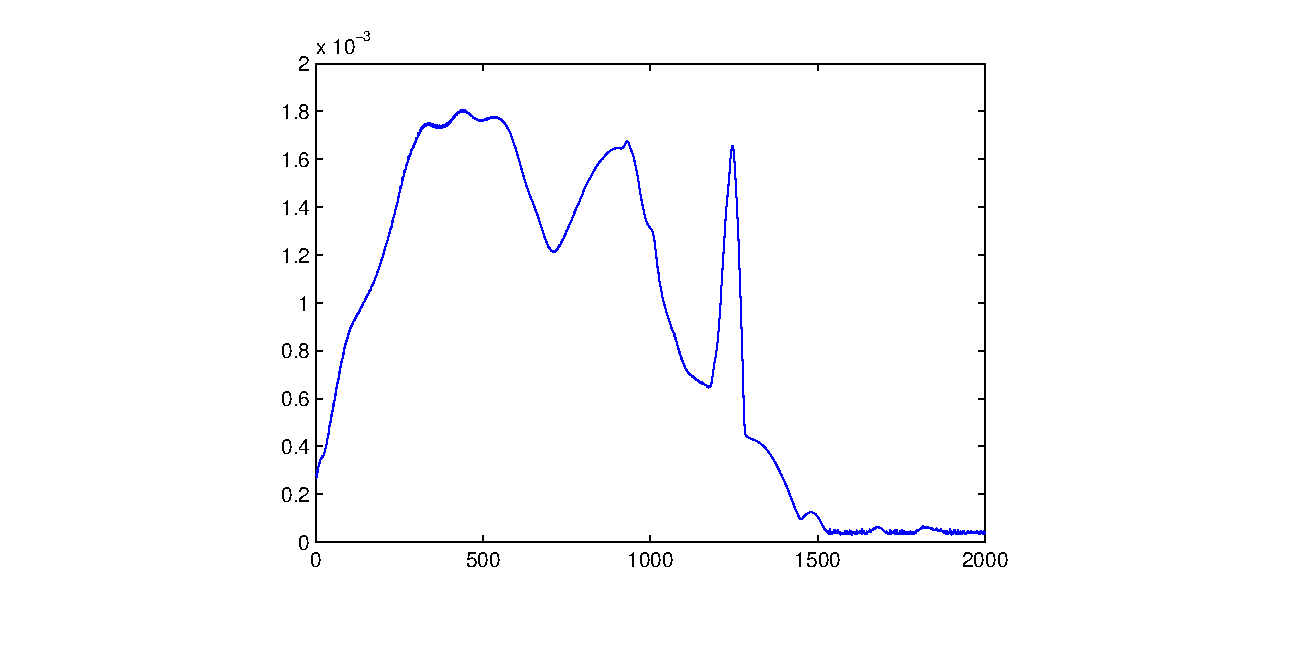
\includegraphics[scale=0.7]{images/crit_it_rx1_t1.eps}
\caption{$||{\phi_{n+1}-\phi_n}||$ according to the number of iteration, for rx1 picture}
\label{fig1}
\end{figure}

\begin{figure}[H]
\centering
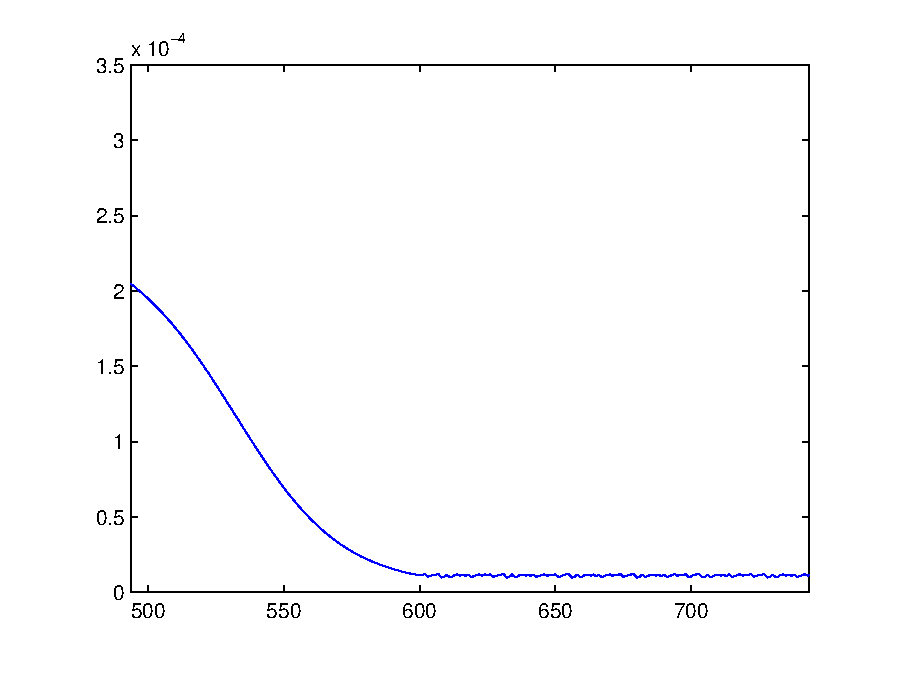
\includegraphics[scale=0.7]{images/crit_it_rx2_t1_zoom.eps}
\caption{$||{\phi_{n+1}-\phi_n}||$ according to the number of iteration, for rx1 picture}
\label{fig2}
\end{figure}

$S_1 = ||{\phi_{n+1}-\phi_n}||$ can't be taken as a stopping criterion. This value stabilise at around $10^-4$ for rx1 (see figure~\ref{fig1}), $10^-5$ for rx2 (see figure~\ref{fig2}). So it is hard to define a tolerance.
Then we decided to choose as a stopping criterion the derivative of $S_1$, filter by a low pass filter (to suppress oscillation effect, see figure~\ref{fig3}). The algorithm stop if $\frac {dS_1} {dn} < tol$ over 20 iterations. 
Oscillations can be explain by the fact that $c_1$ and $c_2$ depends on $\phi$, but doesn't appear in descent term, so a sightl error is introduced which prevent the algorithm to totally stabilise.

\begin{figure}[H]
\centering
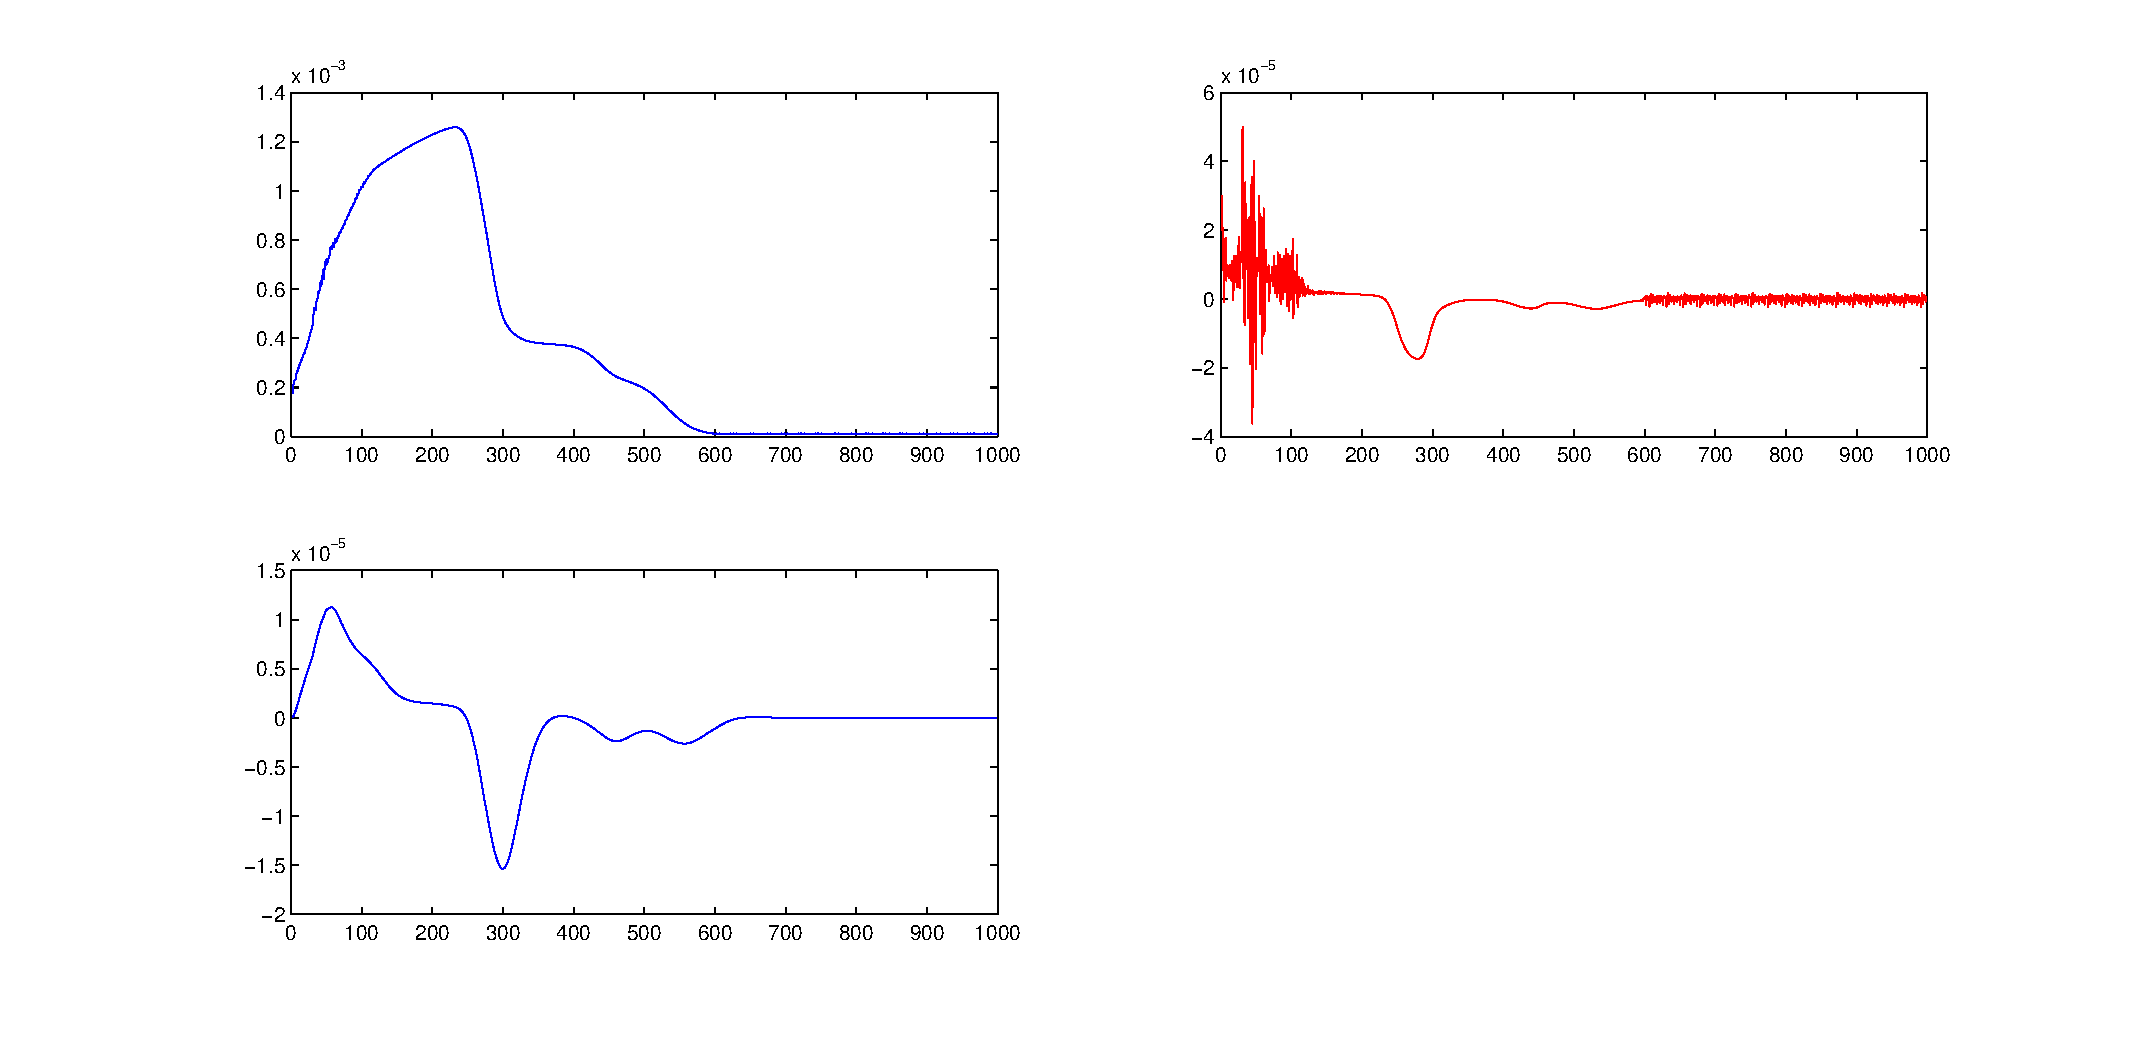
\includegraphics[scale=0.4]{images/crit_it_rx2_t2.eps}
\caption{From left to right : $S_1$, its derivative, and its filtered derivative}
\label{fig3}
\end{figure}

\subsection{Tests}

As Euler-Lagrange equation can only ensure a local minimum, the algorithm depends on initialisation.
It also depends on coefficients $\alpha$ relative to $\lamba_1$ and $\lambda_2$. We set $\lambda_2 = 1$ for the tests.
Figures % TO COMPLETE 
in annexes shows the result depends on whole parameters.
Moreover goods results may be obtain for different parameters on two pictures.
The work to be described further is try to automatise the algorithm (reduce or even suppress the parameters dependency).

\subsection{Local segmentation}
\textit{See section \ref{localcode} for the \texttt{MatLab} code}.\\
A way to really improve the active contour method for more heterogeneous picture, like radiography, is to use local statistics instead of global statistics in the algorithm. Indeed, we can see in figure \ref{interestLocal} that the bottom of the tooth has almost the same shade of gray than some part of the gum. So the global method won't be able to distinguish those two parts of the radiography. The key here is to not examine those two parts together, and instead, examine each pixel of the radiography locally. In other words, at each iteration of the algorithm, instead of having statistics about the whole picture, we create a small ball centred on the current pixel and calculate the same statistics but inside the ball. For further information, see \cite{lanktonLO}. 

\begin{figure}[H]
\centering
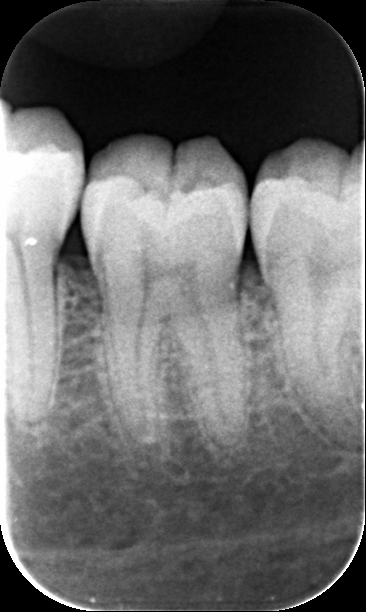
\includegraphics[scale=1.8]{images/rx1.png}
\caption{Interest of the local active contour method : bottom of the tooth has the same shade of gray as some part of the gum}
\label{interestLocal}
\end{figure}

In the following (see the next two figures), we create another initialisation for the active contour method by using two ellipses, one around the tooth and one between the two roots. So that if we take the area between the two ellipses, we can have a pretty good initialisation. Here is an example of the improvement brought by the local method compared to the global method (we used the exact same parameter and the same number of iteration): 
\begin{figure}[H]
\centering
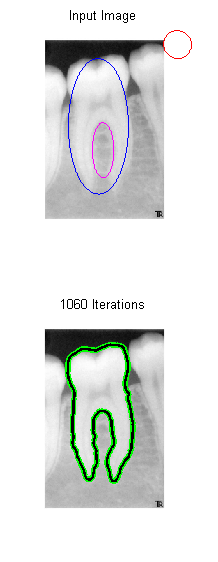
\includegraphics[scale=0.8]{images/doubleEllipseTest_rx2.png}
\caption{Segmentation with the local method : Red circle has the same radius as the ball used in the algorithm. The two ellipses are used for the initialisation.}
\label{ellipseLO}
\end{figure}
As we can see, the segmentation is here almost perfect with the local algorithm. Segmentation with the region based active contour method is behaving as expected : since the tooth shade of gray is almost the same as the gum, the algorithm cannot separate them (see figure \ref{ellipseGLO}). However, local algorithm is really slow since we have to consider each pixel around the zero level set of $\phi$ and calculate statistics of pixels in the ball centred on the first pixel. The total execution time of the local algorithm was about 20 minutes on this high definition radiography while the global method execution time was barely 30 seconds. To improve the local algorithm, we have to use another way to implement the level set function $\phi$. The best is the sparse field method proposed by Whitaker (see \cite{whitaker} for more details). The author of \cite{lanktonLO} implemented this method on the local algorithm and it did save a lot of computations (see \cite{lanktonSFM}).     
\begin{figure}[H]
\centering
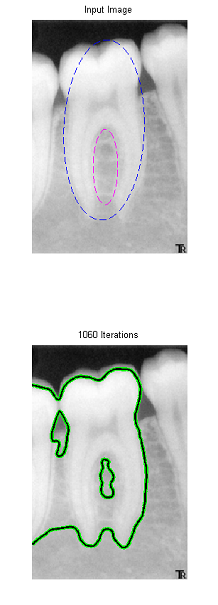
\includegraphics[scale=0.8]{images/doubleEllipseTest_rx2_region.png}
\caption{Segmentation with the global method : bad segmentation between the two teeth.}
\end{figure}




\newpage
\section{Differents way to decrease parameters dependency}
We experimented some ways to reduce initialisation, $\alpha$ and $\lambda_1$ dependency. Those are described in the following sections.

\subsection{Clustering initialisation}
\textit{See section \ref{clusteringcode} for the \texttt{MatLab} code}.\\
Clustering aims at sorting pixel of the radiography into a certain number of cluster. If we look closely to the radiography histogram (see figure \ref{rx2histo}), we can see three peaks : the tooth (white), the gum (gray) and the background (black). 
\begin{figure}[H]
\centering
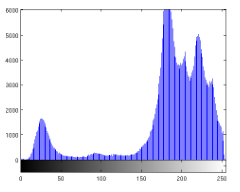
\includegraphics[scale=0.7]{images/rx2histo.png}
\caption{rx2 radiography histogram}
\label{rx2histo}
\end{figure}

As we have seen previously, the initialisation in the active contour method is very important and it could be very interesting to have a mask already almost on the tooth. So clustering the radiography in three parts in order to extract the most we can of the tooth could make the Chan-Vese method works better. In the following, we will talk about the clustering algorithm we have been working on : the k-means and the Otsu algorithm. 
\subsubsection*{Quick explanation of the k-means algorithm}
We have a set of $(x_{i})_{i=1..n} \in \mathbb{R}^p$, we want to classify them in k clusters. We note $\Pi = (\pi_{j})_{j=1..k}$ the k clusters and $m_{j} = \frac{\sum\limits_{l\in\pi_{j}}x_{l}}{|\pi_{j}|}$ the mean or centroid of the cluster j . The aim of k means is to minimise the sum of the distance between each point in the cluster and its centroid on every cluster : 
\begin{equation}
\centering
\inf\limits_{\Pi} \sum_{j=1}^{k} \sum\limits_{l\in\pi_{j}}\norm{x_{l}-m_{l}}
\label{kmeansformula}
\end{equation}

The k means algorithm is a heuristic and is described in the following :
\begin{itemize}
\item Start with k centroid and calculate the corresponding error.
\item For each pixel in the radiography, find the closest centroid and put that pixel in the centroid's cluster.
\item Calculate the new error : if the difference between the new error and the old is less than $tol$, then stop, else go back to the second step
\end{itemize}
As we can see, the k means is really dependent on the initialisation : different runs of k means can have different outputs. The Global K-means algorithm is another algorithm using the local k mean descirbed above and does not depend on the initialisation. The basic idea of global K means is that the best solution for clustering an image into M clusters can be found from the solution of the M-1 clustering problem. However, Global K means cost a lot more in term of space and time. For more information about Global K means, see \cite{gkmeans}. The multi-level thresholding Otsu method is based on the Otsu method which minimise a certain variance to sort pixel in different cluster. It is equivalent to K means algorithm, that's why we won't use it in the following. \\
\subsubsection*{K means with radiography}
By using K means, or global K means, we can now cluster pixel of the radiography in three parts and extract the part corresponding to the tooth. However, we have to choose a norm for formula \ref{kmeansformula}. We have choose to compare three different norms ( we note (i,j) coordinates of a pixel and $I_{ij}$ its gray intensity) :
\begin{itemize}
\item The $L_{1}$ norm or City Block norm : $|I_{ij}-I_{i'j'}|$
\item The $L_{2}$ norm or Euclidian norm : $\norm{I_{ij}-I_{i'j'}}$
\item Since the last two norms only consider the gray intensity, we could think of a norm taking the geometry into account.
\begin{equation}
\alpha \times d((i,j),(i',j')) + \beta \times \frac{|I_{ij}-I_{i'j'}|}{255}
\end{equation}
where $\alpha$ and $\beta$ are parameters
\end{itemize}
Several tests have shown that the third norm isn't really interesting since the best value for $\alpha$ is 0.05 and 0.95 for $\beta$, so geometry isn't important in this problem. Moreover, the first norm is often better for what we have to do. For instance, on the figure \ref{interestnorm} below, a biggest part of the tooth is detected (left) than with the second norm (right).
\begin{figure}[H]
\centering
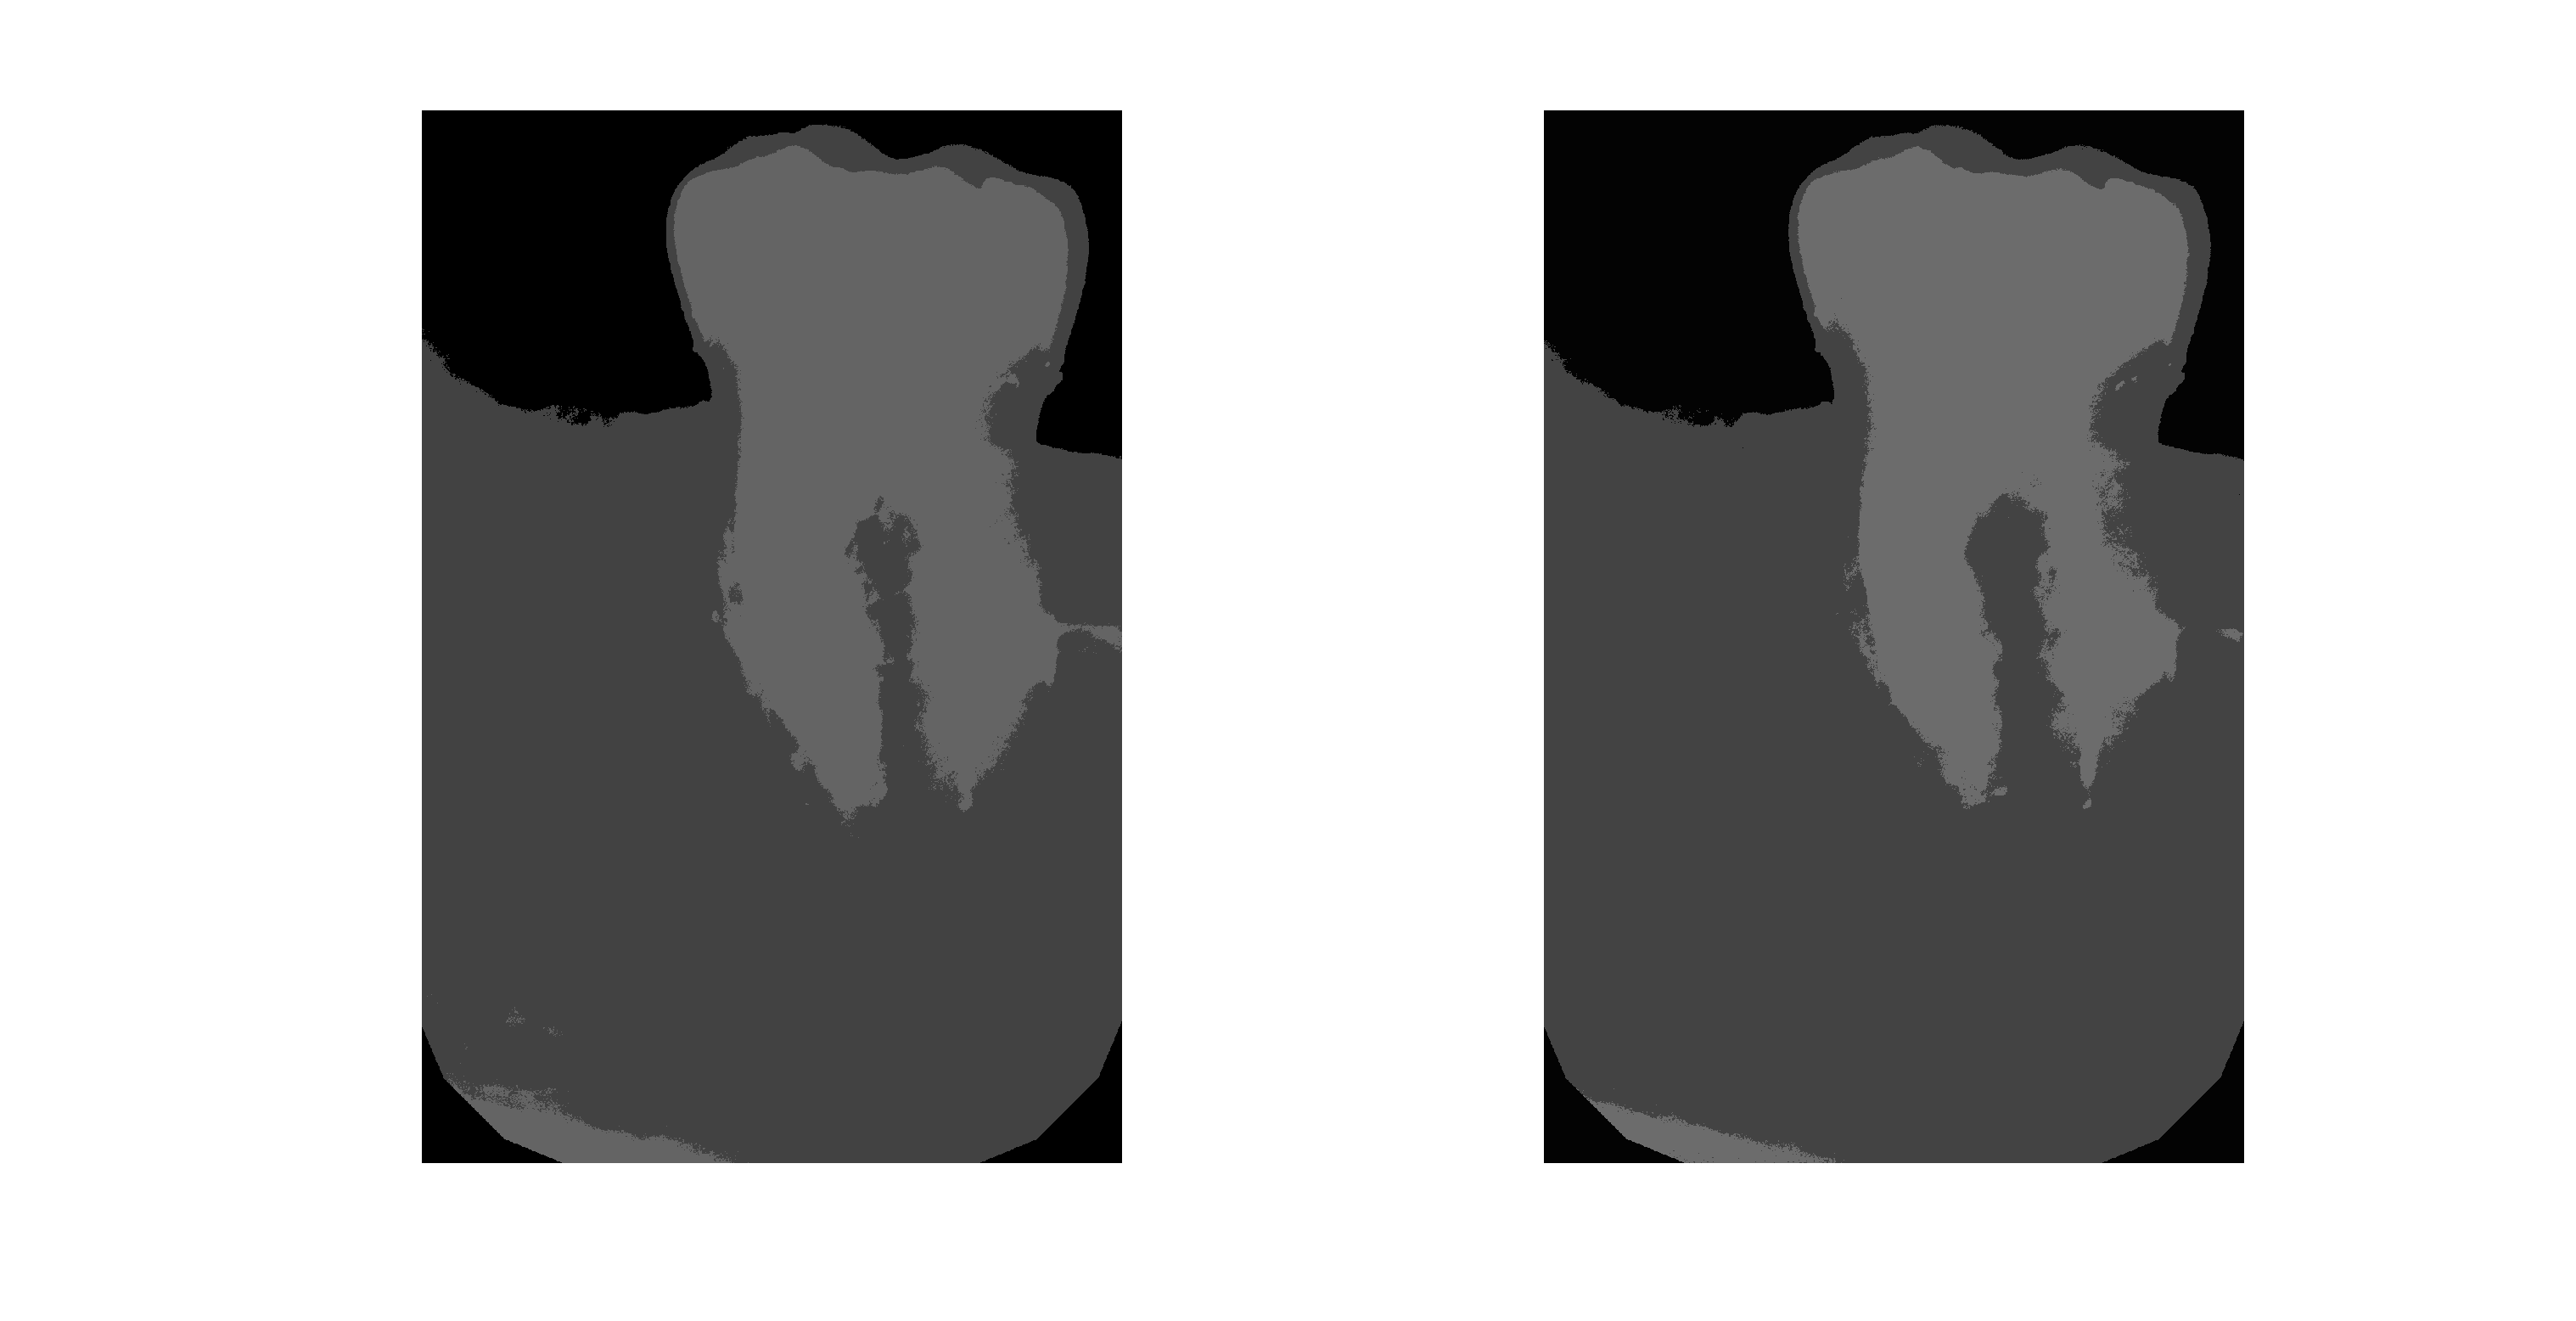
\includegraphics[scale=0.3]{images/normkmeans.eps}
\caption{Run of kmeans with norm 1 (left) and norm 2 (right)}
\label{interestnorm}
\end{figure}

In the following, we only use the first norm (city block norm or $L_{1}$ norm). We choose to use always four clusters to extract the tooth instead of three : indeed, in some radiography, there is a part inside the tooth with a different shade of gray. So if we take only three clusters, we might miss the tooth (see figure \ref{numberCluster})

\begin{figure}[H]
\centering
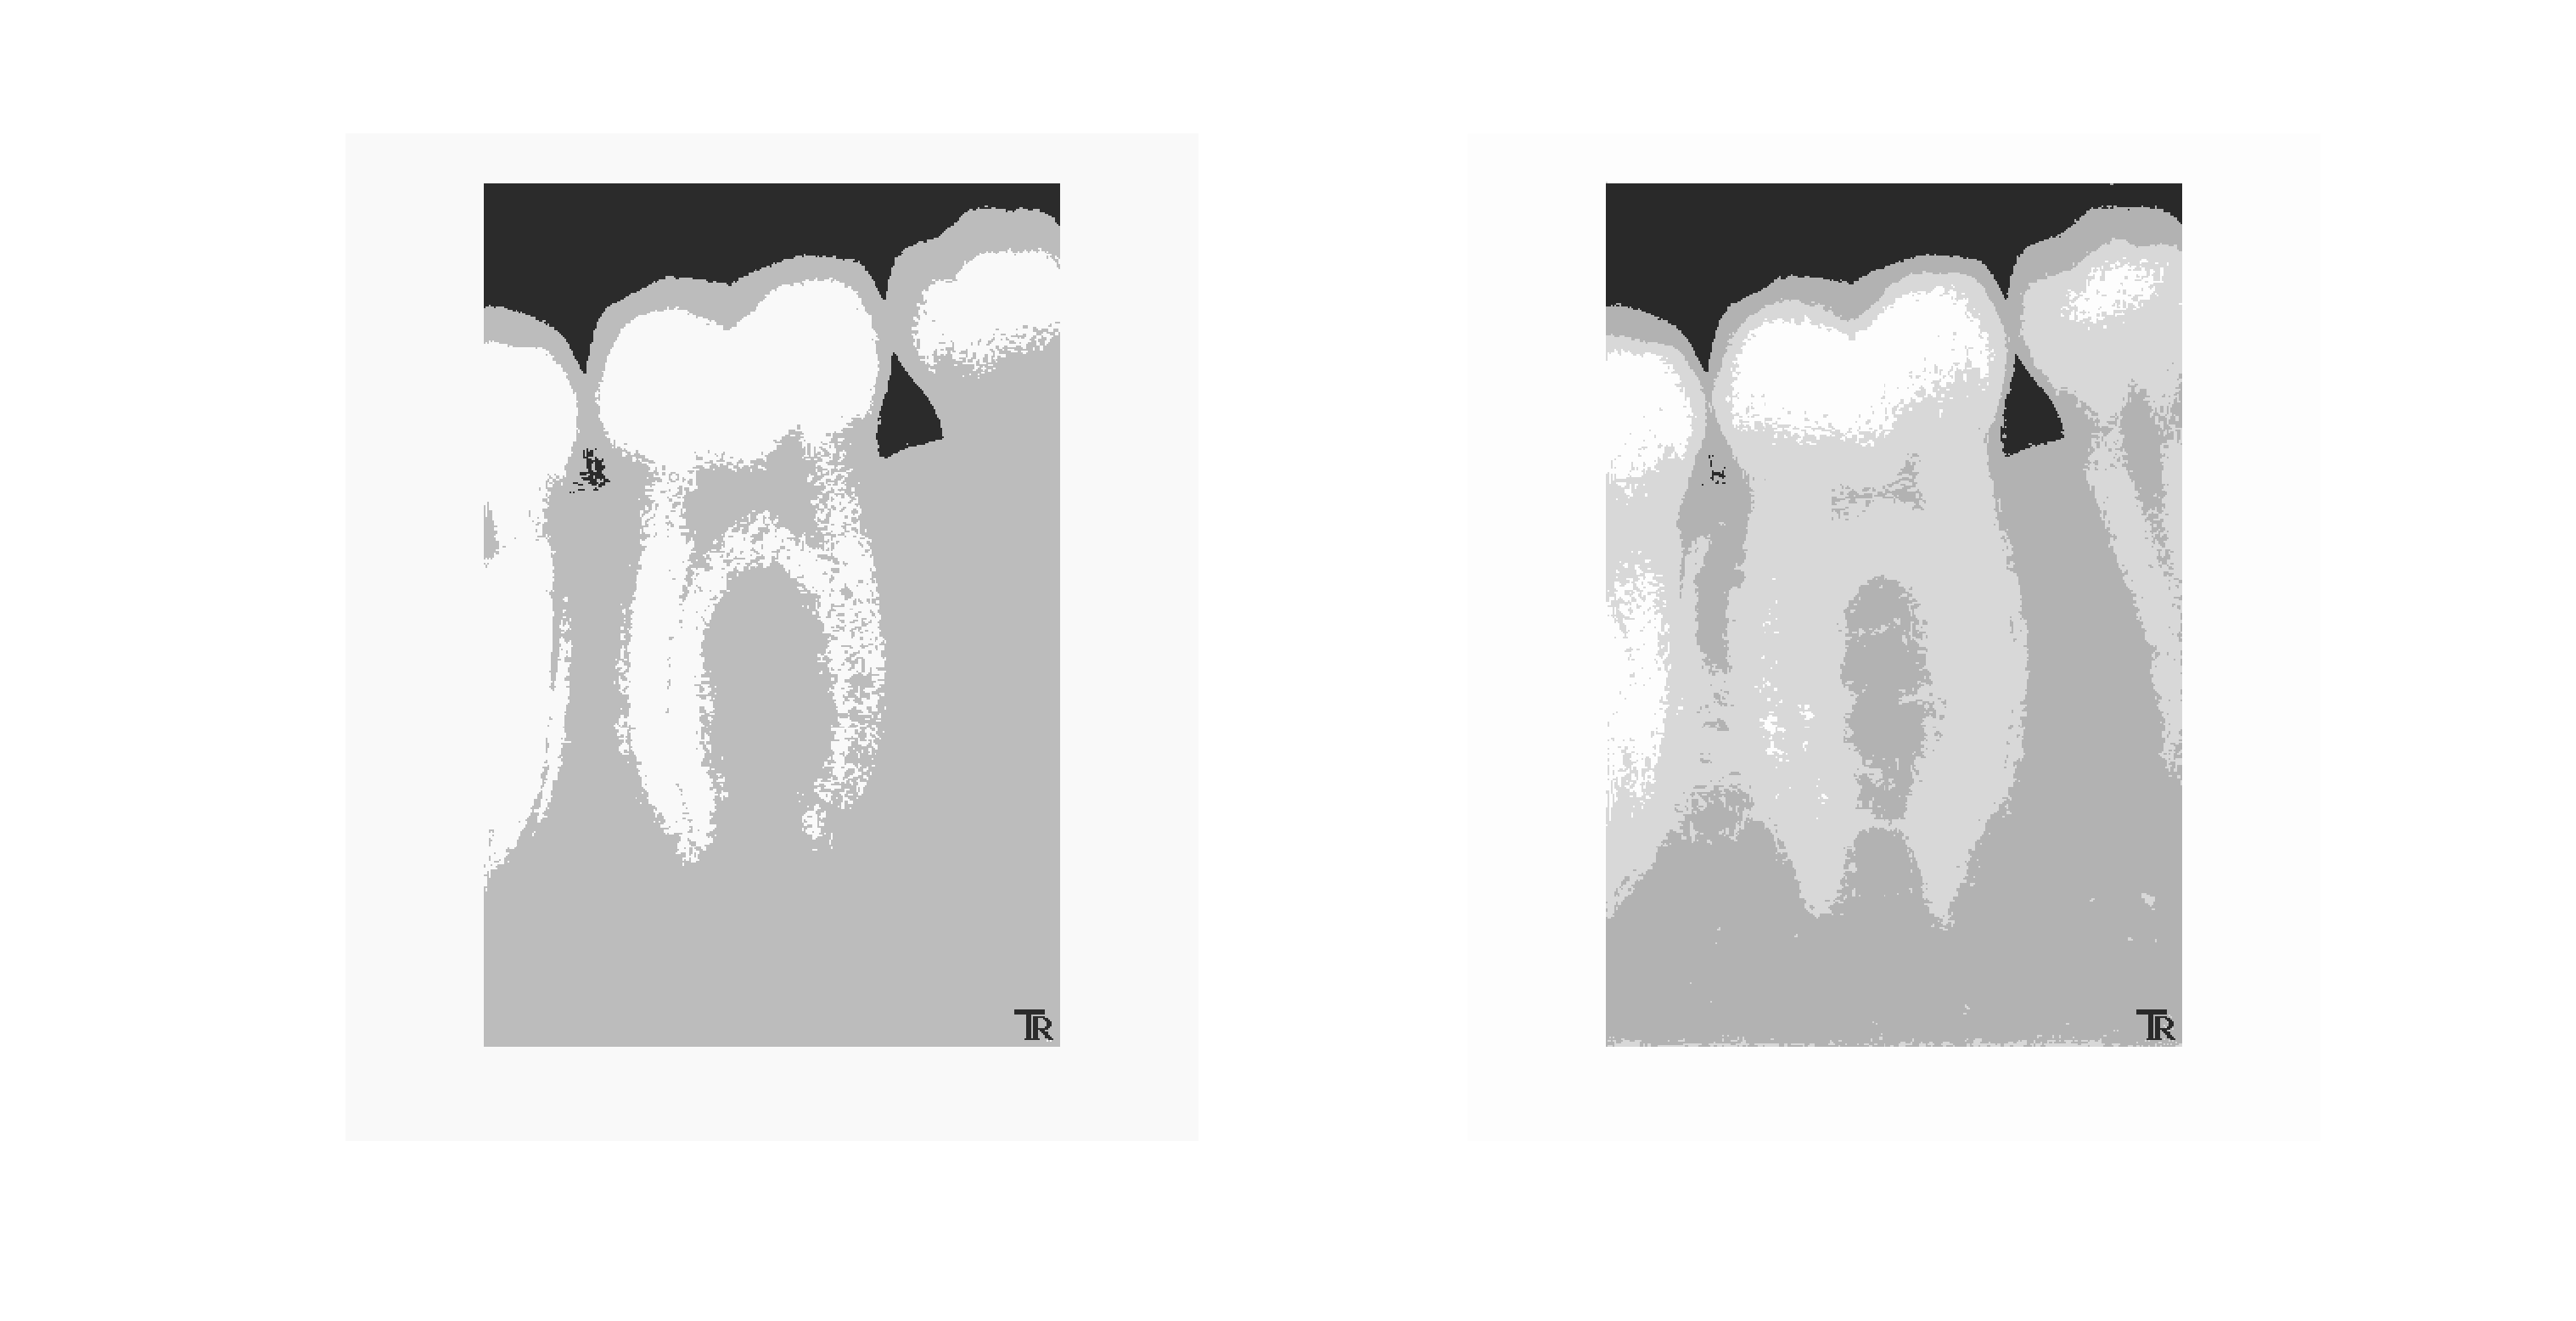
\includegraphics[scale=0.3]{images/numberCluster.eps}
\caption{Number of cluster : 3 in the left and 4 in the right}
\label{numberCluster}
\end{figure}

For the active contour method initialisation we need a black and white mask. After clustering the radiography in four parts, we know that the two lightest part are the part corresponding to the tooth since the two others are the gum and the background : those two parts are going to be white, the others will be black. Here is the output of the execution of the algorithm on different radiography :

\begin{figure}[H]
\centering
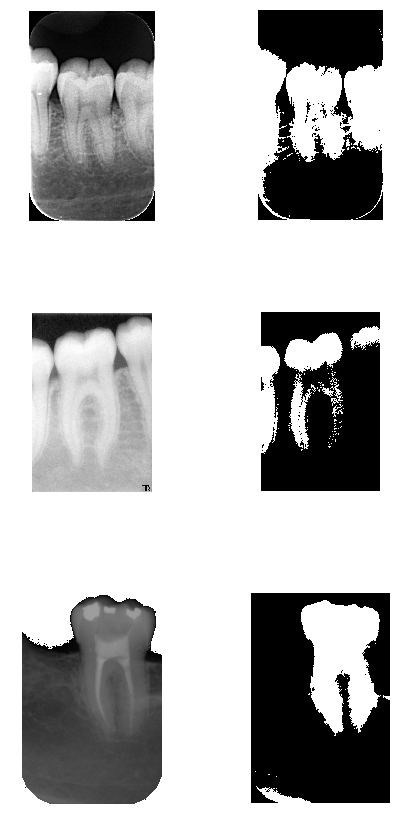
\includegraphics[scale=0.6]{images/clusterRun.png}
\caption{Extraction of the tooth : in the left the original radiography, in the right the mask.}
\label{cluster}
\end{figure}

As we can see, clustering is not perfect : there are still a lot of noises where the gum is. That's what motivated us to use the PCA method to extract the gum before using clustering in section 3.3.1.
\subsection{Curve guidance}

According to figures  the $\alpha$ parameter influence the final shape. A too big $\alpha$ will make the algorithm extract a part of a tooth only, when a too small $\alpha$ lead to an unsmooth curve (which might includes gum's nerves), or will extract many tooth.  

In order to fix this issue, we introduce a new term in Chan-Vese energy F. The idea is to add a gravity energy term, guiding the curve into a hole (some holes) around the tooth (by minimising the gravity energy).

\subsubsection*{Guide the curve to a predefine contour}

We assume we have a contour $C_{ap}$ approximately fitting the curve. We then add a surface gravity energy to Chan-Vese energy, compute over $Inside(C_{ap})$
We had to add to (\ref{cv_energy}) the term :

\begin{equation}
\begin{split}
    E_p &= \frac{1}{\text{Area}(C)} \int_{inside(C)} e(x,y)dxdy \\ &=  \frac{1}{\text{Area}(C)}\int_{\Omega} e(x,y) H(\phi(x,y))dxdxy 
\label{area_energy}
\end{split}
\end{equation}

Where $e(x,y)$ is a surface energy field, negative inside $C_ap$ (push the active contour to the outside), positive outside (push the active contour to the inside).

We compute the Area($C$) at each iteration (as for $c_1$ and $c_2$). \\
Then applying the Euler-Lagrange formula to \ref{area_energy} add to \ref{descent_direction} the simple term $e(x,y)$
We compute $e(x,y)$ as the square of the distance to (x,y) from $C_{ap}$

Figure~\ref{without_hole} shows the Chan-Vese algorithm application without hole, figure~\ref{with_hole} the computation with a rectangular hole around the tooth. The result isn't better (as the hole is rectangular), but the goal (preventing the curve to leave the tooth for a too small alpha) is reached. Moreover the computation speed increase. 

\begin{figure}[H]
\centering
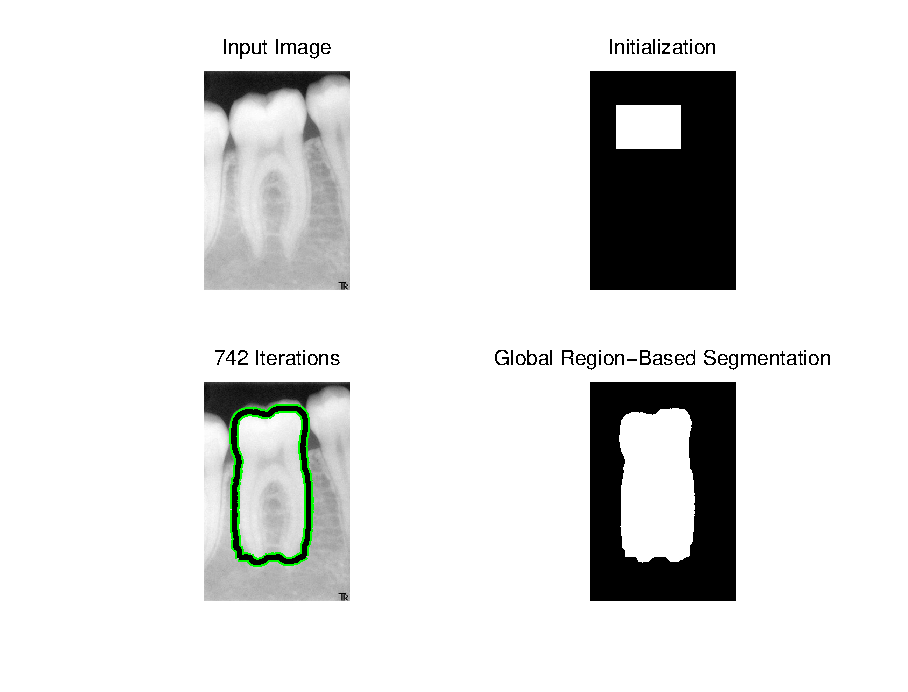
\includegraphics[scale=0.7]{images/with_hole_rx2.eps}
\caption{Computation with a rectangular $C_{ap}$ hole around the tooth}
\label{with_hole}
\end{figure}

\begin{figure}[H]
\centering
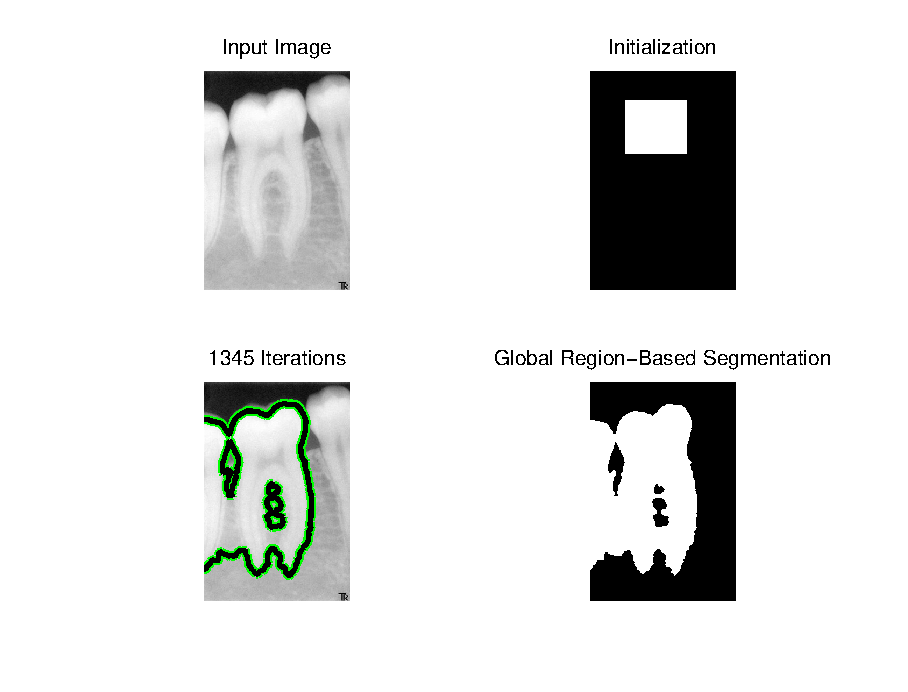
\includegraphics[scale=0.7]{images/without_hole_rx2.eps}
\caption{Computation without the rectangular $C_{ap}$ hole around the tooth}
\label{without_hole}
\end{figure}

\subsubsection*{Guide the curve to control points}

The idea is the same than in the previous part, but here we compute a linear gravity energy along C.
We had to (\ref{cv_energy}) the term : 

\begin{equation}
\begin{split}
    E_p &= \frac{1}{\text{Length}(C)} \int_{C} e_l(x,y)dC \\ &\approx \frac{1}{\text{Length}(C)} \int_{\Omega} e_l(x,y) \delta_{\epsilon}(\phi(x,y)) |\bigtriangledown \phi(x,y)| dxdxy 
\label{linear_energy}
\end{split}
\end{equation}

Where $e_l(x,y)$ is a linear energy field, such as $\textcursive{M} = min(e_l(x,y))$ is the set of required control points. Then the curve should be "attracted" by those control points. 
\\The energy (\ref{linear_energy}) add to (\ref{descent_direction}) the term :

\begin{equation}
    \frac{\partial e_l}{\partial x}.\frac{\partial \phi}{\partial x} \ + \ \frac{\partial e_l}{\partial y}.\frac{\partial \phi}{\partial y}
\end{equation}

The implementation doesn't work so far, so we have no tests to propose. This method is only reported here for information.





\subsection{Image pre-treatment}  
\subsubsection*{Texture analysis by PCA}
\textit{See section \ref{pcacode} for the \texttt{MatLab} code}.\\
As seen previously, the gum is causing a lot of trouble in active contour algorithm. In radiography of our database, the gum between teeth is like noise preventing the good behaviour of almost every of our algorithm (as shown below in figure \ref{noisePCA} showing gum noises between teeth). Thus, our goal here is to get rid of the gum by using some of its characteristics.
\begin{figure}[H]
\centering
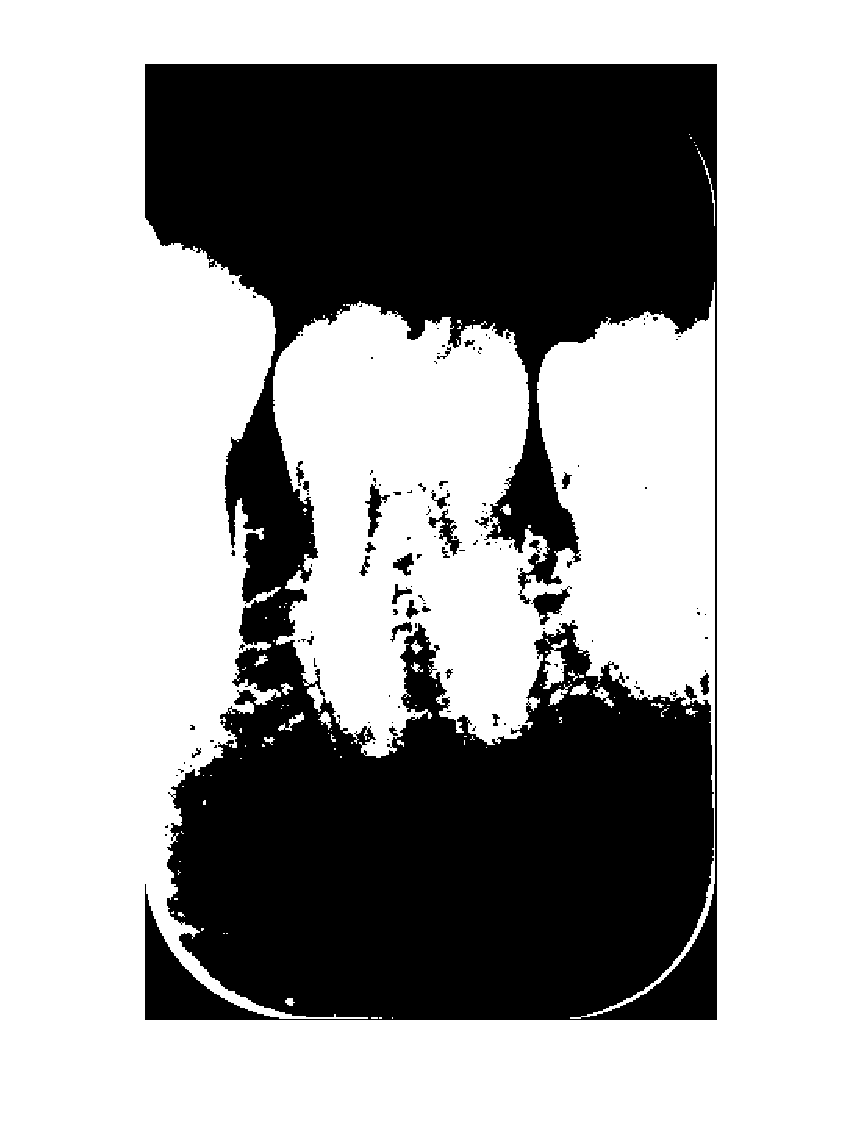
\includegraphics[scale=0.5]{images/noisePCA.eps}
\caption{Noises between teeth caused by gum in k-means clustering}
\label{noisePCA}
\end{figure}
Our first idea was to use the gum pattern to recognise and search the gum in radiography. To do that, we are using principal component analysis. The PCA is based on a pretty simple idea : starting with a set of $p$ points in $\mathbb{R}^n$ (or p subjects defined by n varibles), we want to find vectors explaining the maximum variability of those points. Those vectors are actually really simple to find. Indeed, if we note $X_{c}$ the p x n matrix filled with the previous points minus their means, then it is easy to show that those vectors are eigenvectors of the matrix $X^{t}_{c}X_{c}$, each vector explaining a certain variability depending on the size of the associate eigenvalue.\\ We will be using the PCA on the gum to find its characteristics and to be able to recognise it. To do so, we are applying the same algorithm on each picture of our database :
\begin{itemize}
\item Select a square in the gum pattern
\item Split this square in $p$ little bloc of size $\omega\times\omega$ . $\omega$ must be big enough to have enough pixel and small enough to not have big basis.
\item Each bloc of $\omega ^2$ variables is a subject in the PCA so that the matrix sized used is $p\times \omega ^2$. Then, the PCA gives us a basis of bloc of $\omega ^2$ vectors of size $\omega ^2$ explaining the maximum variability of those blocs. We can then use this basis to rebuild the whole radiography by splitting the image in blocs of size $\omega$ and by projecting all of those blocs on the first vector of this basis, since it's the one explaining the most of the variability. 
\end{itemize}

We know how to build a basis of bloc for each pattern of the radiography, hence, we do that for the gum, the tooth and the background. In our problem, we have to recognise and sort all the bloc by their texture. Thus, we select a bloc of the picture. In the following, we note $I_{proj}$ the projection of the bloc on the first k basis vectors, $(B_{i})_{(i=1..nText)}$ the nText pattern bloc basis where nText is the total number of texture. Thus, the projection of the bloc I on the basis $B_{j}$ is :
\begin{equation}
\exists (\alpha_{1},\alpha_{2},...,\alpha_{k}) \in \mathbb{R}^k , I_{proj} = \sum_{j=1}^{k} \alpha_{j} \times B_{j}(:,j) 
\label{proj_I}
\end{equation}
To sort the bloc I in the right texture, we had two ideas :
\begin{itemize}
\item We project the bloc on each pattern bloc basis $B_{j}$, we calculate the $L_{2}$ norm error $err(j) = \norm{I_{proj}-I}$ and we choose the one basis minimising this error : $min_{j=1 .. nText} err(j)$.
\item We project the bloc on each pattern bloc basis $B_{j}$. Since the projection $I_{proj}$ must not be good on all of the basis except the right one, the projection coefficient must be small on the right texture basis and big on wrong texture basis. Then we choose the basis j such as :  $min_{j=1 .. nText} \sum_{i=1}^{k} |\alpha_{i}|$
\end{itemize}
After several tests, we found out that the second criterion is the best to sort bloc by their texture. For instance in figure \ref{textPCA}, we have three textures and we use the algorithm described above to sort each bloc of the picture by their texture. In the third and fourth part of the MatLab figure, each bloc of the original picture has a gray shade : it is white if it belongs to the texture in the right of the picture, gray if it belongs to the middle texture, dark gray if it belongs to the left texture, depending on the criterion used to sort. In the third part, we use minimisation of the projection coefficient criterion, in the fourth part, we use the minimisation of the error criterion. Since we know the obvious answer of the sorting, we can compare which method is the best.  
\begin{figure}[H]
\centering
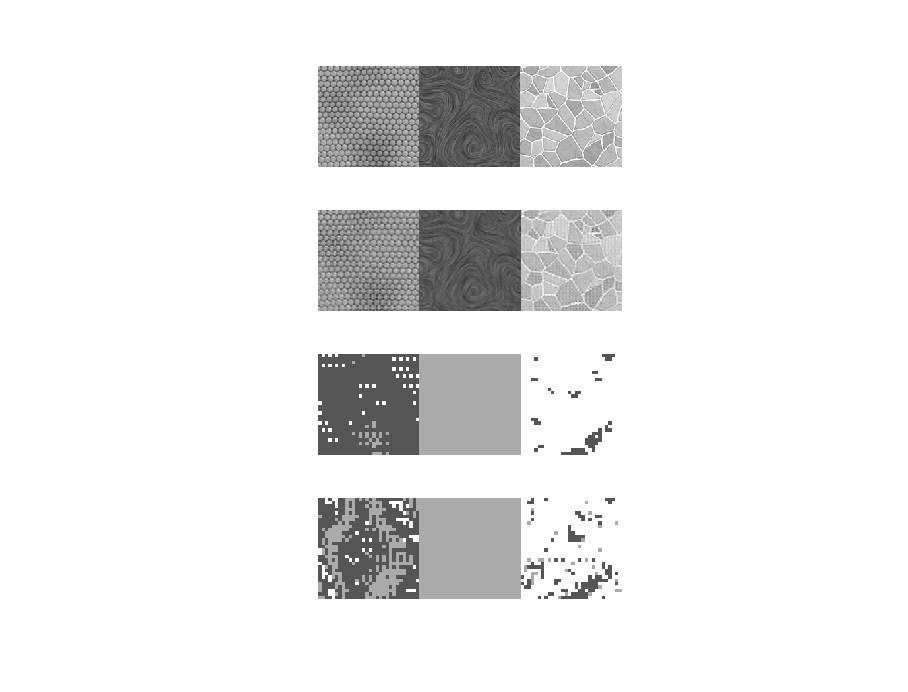
\includegraphics[scale=1]{images/testMethodeSegPCA.eps}
\caption{Sorting bloc by their texture with PCA}
\label{textPCA}
\end{figure}
Once we have the criterion to sort bloc by their texture, we can build a database of gum texture to be able to sort the gum of every kind of radiography. We started by building it with five radiography, and we tried to run the sorting algorithm on other radiography found on the internet. Here are the results of our tests (in white the gum, in black the other part) :
\begin{figure}[H]
\centering
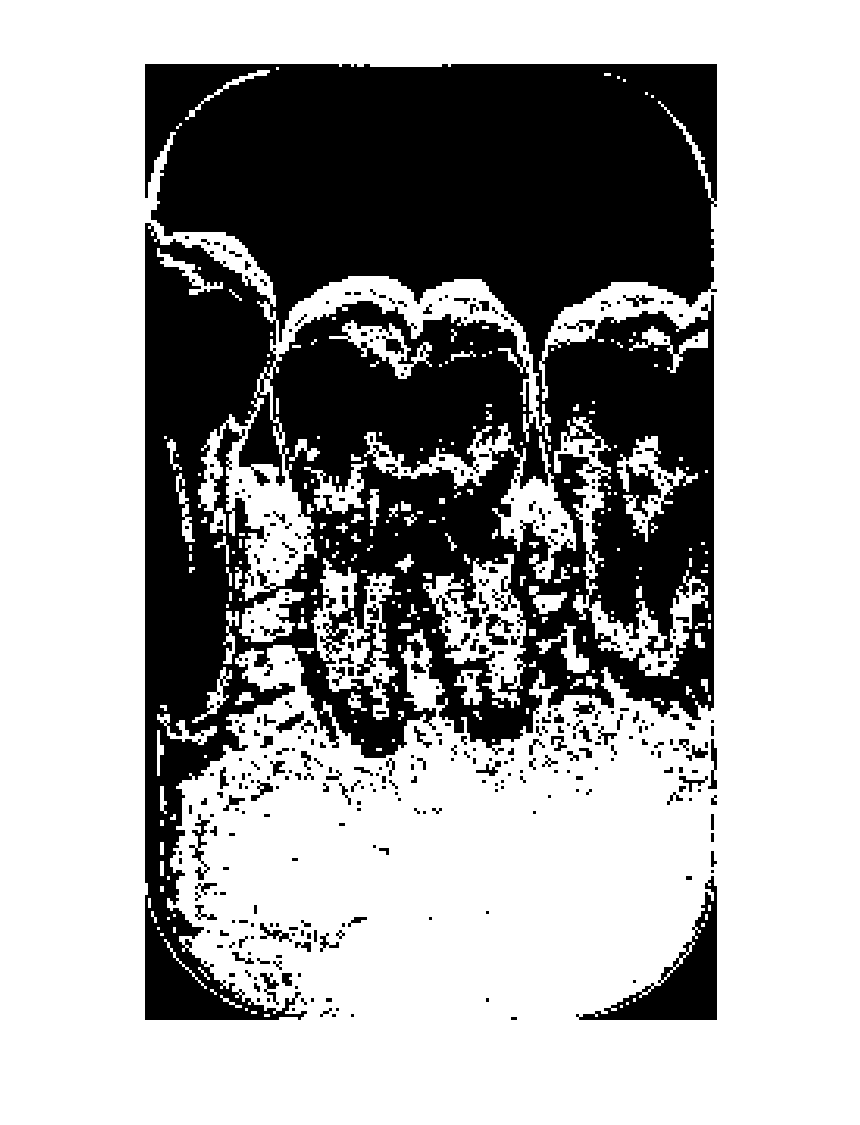
\includegraphics[scale=0.3]{images/recTextrx1.eps}
\caption{in white the gum, in black the other part}
\label{recText}
\end{figure}
The sorting is not really well working when we use data from our database. This might be caused by too many different shade of gray in the radiography used to create the database since the sorting is pretty well working (see figure \ref{testDentPCA}) when using basis extracted directly from the radiography, and not from other database basis. 
\begin{figure}[H]
\centering
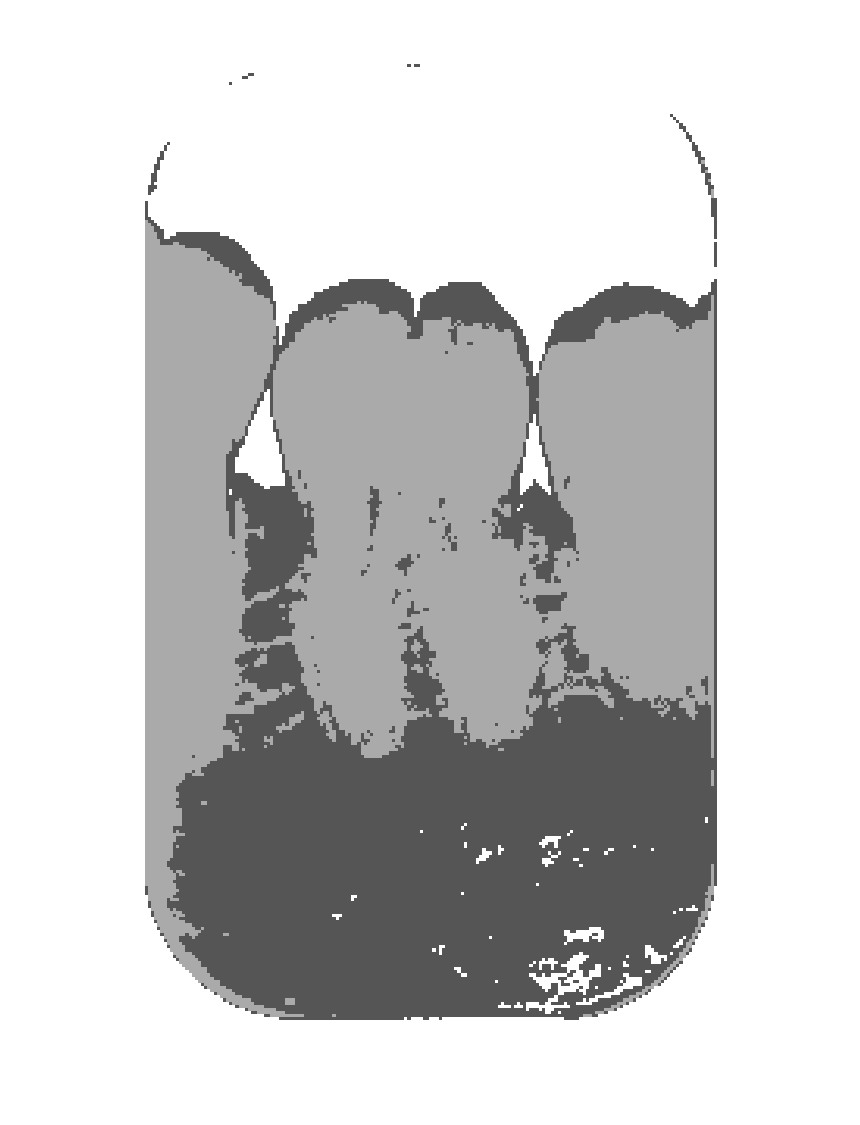
\includegraphics[scale=0.3]{images/testDentPCA.eps}
\caption{Sorting using only basis calculated from the radiography}
\label{testDentPCA}
\end{figure}

\subsubsection*{Different modification on the original image}

We tried different simple pretreament on the image.
Only two showed off some results.
The first is to black the image away from an aproximate mask fitting the tooth. As Chan-Vese need to compute inner and outter intensity means, the goal is to avoid some perturbation due to picture's parts which have the same color as the tooth. Figure (\ref{blackrx2}) show the black rx2 image. Figure (\ref{withoutblack}) and  (\ref{withblack}) show how this can reduce the $\alpha$ dependency. Indeed as the curve isn't attracted by the others tooth or nerves in gum, the curve is smoothest, without the need to increase $\alpha$

\begin{figure}[H]
\centering
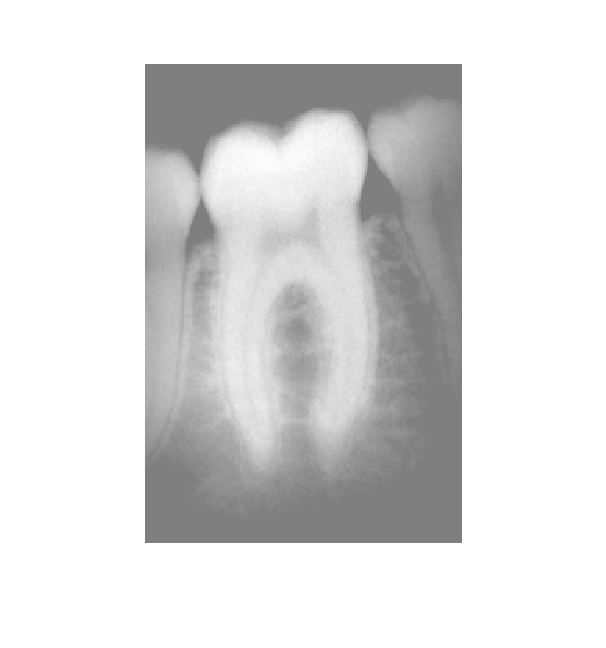
\includegraphics[scale=0.7]{images/blackrx2.eps}
\caption{Black rx2.jpg}
\label{blackrx2}
\end{figure}

\begin{figure}[H]
\centering
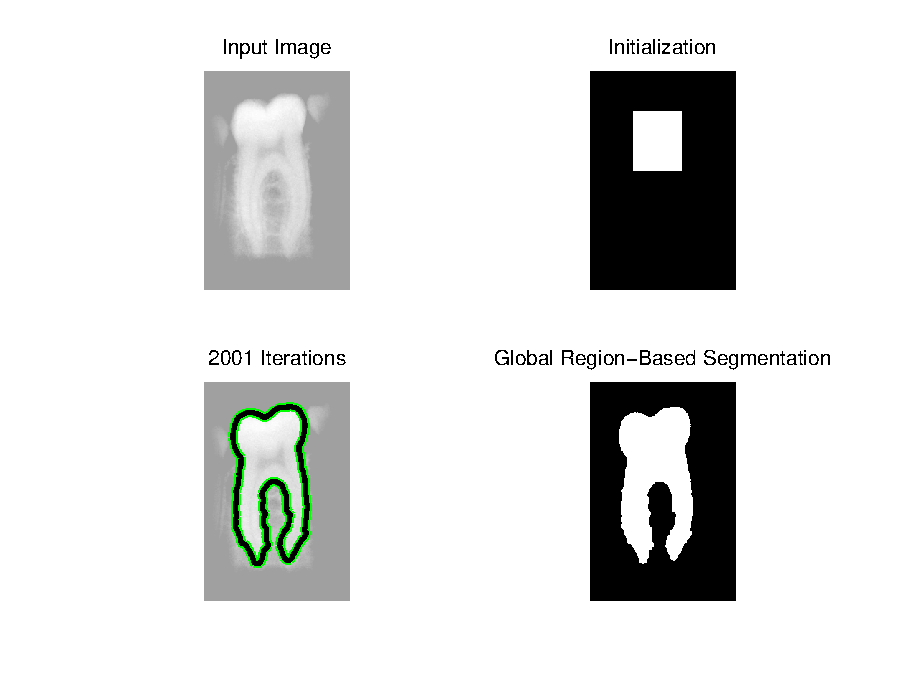
\includegraphics[scale=0.7]{images/cvonblackrx2.eps}
\caption{With blackening}
\label{withblack}
\end{figure}

\begin{figure}[H]
\centering
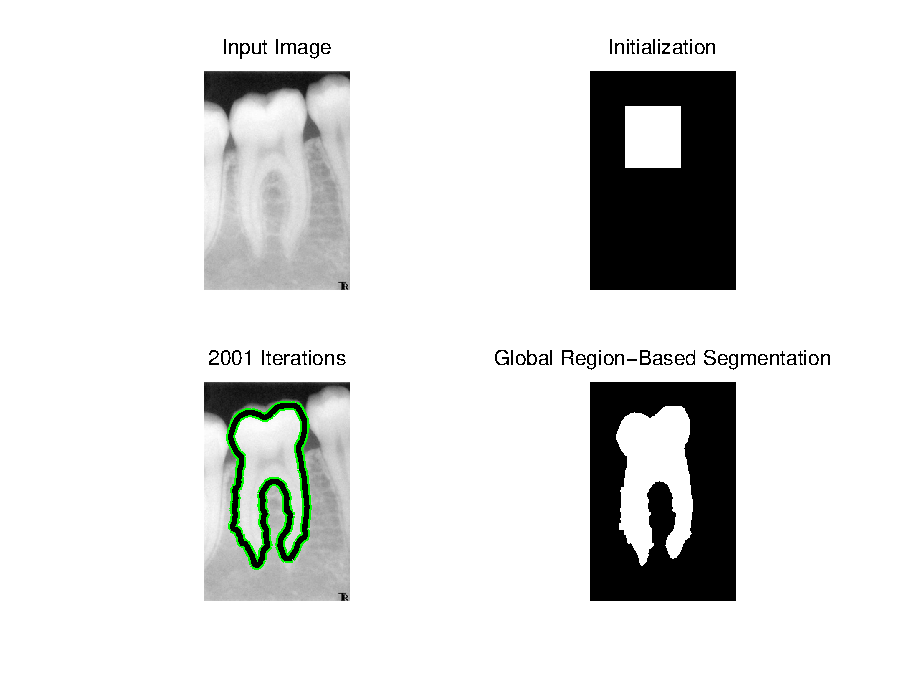
\includegraphics[scale=0.7]{images/cvonnonblackrx2.eps}
\caption{Without blackening}
\label{withoutblack}
\end{figure}

The other pretreament is to blurring the picture, in order to decrease the influence of gum's nerves. Figure (\ref{frx2}) show the result of Chan-Vese on blurred rx2 picture, with $\alpha = 0$. Blur the allows to get ripped of the smooth term. It actually provide a better clustering than Otsu/Clustering methods as it tends to exihibit geometrics "blocks". Though, we still need to initialise the Chan-Vese algorithm on blurred image.

\begin{figure}[H]
\centering
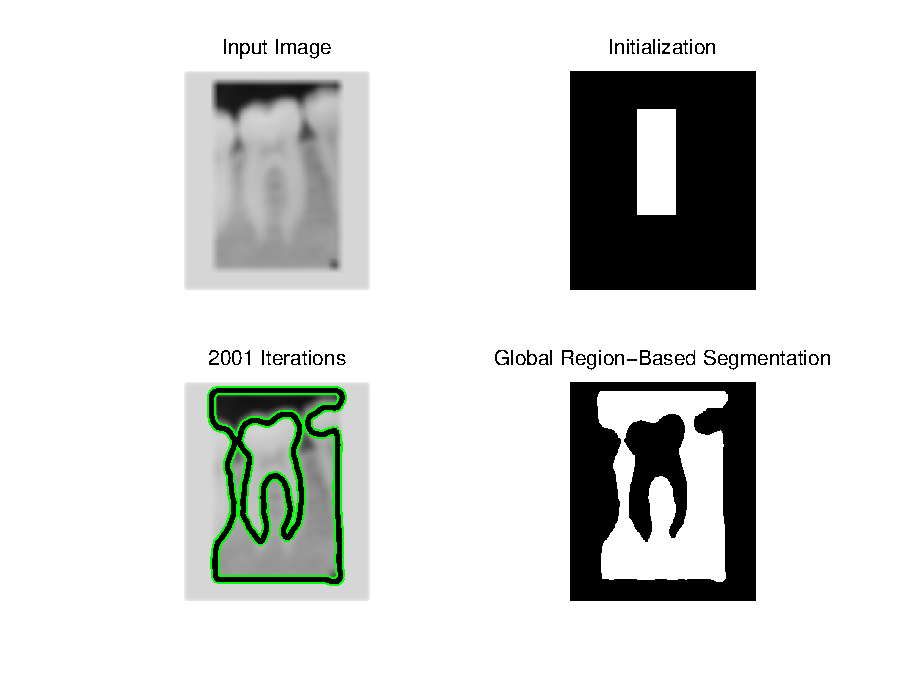
\includegraphics[scale=0.7]{images/flourx2.eps}
\caption{Chan-Vese on a blur image, $\alpha = 0$}
\label{frx2}
\end{figure}





\newpage
% Bonjour Quentin <3 Super utile ce commentaire
%\section{Automation tests}
%\newpage
\section{Appendix}
\subsection{Local Chan-Vese}
\label{localcode}
\subsubsection*{Local Chan-Vese code}
\lstinputlisting{code/localized_seg.m}
\subsubsection*{Demo of the Local Chan-Vese method}
To run the local active contour method demo, write \texttt{localized\_seg\_demo} in the \texttt{MatLab} prompt. You can set different parameters such as the mask initialisation and local method parameters. Here is the code :
\lstinputlisting{code/localized_seg_demo.m}

\subsection{Clustering}
\label{clusteringcode}
\subsubsection*{im2mask}
The first code is \texttt{im2mask.m}, which creates a mask for Chan-Vese initialisation from an image and a method as described in the code documentation. It uses the \texttt{GKmeans.m} file and \texttt{sqdist.m}. You can modify several parameters inside the code of \texttt{im2mask} such as the method used for the clustering (Global Kmeans or MatLab Kmeans), or the number of cluster.    
\lstinputlisting{code/im2mask.m}
\subsubsection*{TestAuto}
\texttt{TestAuto.m} runs an automatic test from an image I and gives the extracted tooth from the Chan-Vese method. 
\lstinputlisting{code/TestAuto.m}

\subsection{Principal Component Analysis}
\label{pcacode}
\subsubsection*{recText}
\texttt{recText} aims at finding the gum in a dental radiography. Its inputs are an image I, and the path to the gum basis matrix and the other parts of the tooth basis matrix. The matrix columns are the vector's bloc basis from the PCA, and the last row is the mean from the set of points used in the PCA. There are already two database (so four matrix) in our Dropbox files : one was created by using three textures on each radiography, the other by using six textures. \texttt{recText} output is a black and white mask (the gum is black, other parts are white). Here is the code :
\lstinputlisting{code/recText.m}
\subsubsection*{TestDent}
\texttt{TestDent} is a script used to create the gum database. First, we select \texttt{nText} regions of texture we want to analyse, then we run the PCA on those regions. We then try to rebuild every bloc of the radiography by projecting those blocs on the \texttt{nText} texture basis created before. Finally, we try to sort each bloc by their texture by using the two criteria described in the PCA section (each texture has its own intensity of gray). In the code, we can modify the number of texture (\texttt{nText}), or the size of a bloc (\texttt{w}) used in the PCA, or the number of basis vector used in the picture reconstruction (\texttt{coeffProj}). Here is the code :
\lstinputlisting{code/TestDent.m}



\newpage
\section{Bibliography}
\begin{thebibliography}{9}

\bibitem{lanktonLO}
  Shawn M.Lankton,
  \emph{"Localised statistical models in computer vision"},
  PHD Thesis,
  Georgia Institute of Technology,
  2009.
\bibitem{whitaker}
  Ross Whitaker,
  \emph{"A level-set approach to 3d reconstruction from range data."},
  International Journal of Computer Vision,
  R. T. 1998.
\bibitem{lanktonSFM}
  Shawn M.Lankton,
  \emph{"Sparse Field Methods - Technical Report"},
  Technical Report,
  2009.
\bibitem{gkmeans}
  Aristidis Likas, Nikos Vlassis, Jakob J. Verbeek,
  \emph{"The global k-means clustering algorithm"},
  The journal of the pattern recognition society,
  2009.



\end{thebibliography}
\end{document}